\documentclass[12pt]{article}
\usepackage{NotesTeXV3}
\usepackage{graphicx}
\usepackage{physics2}
\usepackage{slashed}
\usepackage{longtable}
\usepackage{tabularx}
\usepackage{lineno}
\usepackage{multirow}
\usepackage{cleveref}
\usepackage{subcaption}
\usepackage{placeins}
\usepackage{pdflscape}

\linenumbers


\author{Mathieu Ouillon}
\date{\today}


\begin{document}

\title{{RG-D Common Analysis Note}\\{\normalsize{\itshape Electron and pion cuts for Run Group D}}}
\affiliation{
Mississippi State University\\
}
\emailAdd{ouillon@jlab.org}
\maketitle

\newpage
\pagestyle{fancynotes}


\section{Particle identification and fiducial cuts}
In this section, we detail the particle identification and selection using the CLAS12 detector. We focus on measuring electrons in the forward detector and charged pions in both the forward and central detectors. Particle identification and refined selection follow procedures developed by Run Group A.

Data has been taken from Pass 1 with a beam energy of 10.54 GeV and has been produced with CLAS12 software \href{https://github.com/JeffersonLab/coatjava/releases/tag/13.0.0}{COATJAVA 13.0.0}. The data are available at \texttt{/cache/clas12/rg-d/production/pass1/}.

\subsection{Electron identification}

The electron is typically the first particle required to define an event for physics analysis. To accurately identify electron candidates, a series of selection criteria, or cuts, is applied to detector responses, specifically targeting negatively charged tracks. These cuts are designed to distinguish electrons from minimum ionizing particles (MIPs), such as negatively charged pions ($\pi^-$). Additionally, the Event Builder assigns a classification (\texttt{status}) based on the detector system in which the electron track is located.

In the initial step, the Event Builder assigns electron or positron identification ($e^- \rightarrow 11,e^+ \rightarrow -11$) to tracks that exhibit appropriate responses in both the High Threshold Cherenkov Counter (HTCC) and the Electromagnetic Calorimeter (ECAL), following the criteria outlined in \cref{tab:electron-requierement}. Additionally, the EB requires an associated matched hit in FTOF, either in panel-1b or, if there is no panel-b hit, in panel-1a.


\begin{table}[hbt]
  \centering
\begin{tabularx}{\textwidth}{|l|l|X|}
\hline
\multicolumn{1}{|c|}{\textbf{Cut}} & \multicolumn{1}{c|}{\textbf{Requirement}} & \multicolumn{1}{c|}{\textbf{Purpose}} \\ \hline
Charge                             & $Q = -1$                                   & Select negative tracks                \\ \hline
HTCC Photoelectrons                & $N_{\text{phe}} > 2$                       & Reject charged hadrons                \\ \hline
PCAL Energy                        & $E_{\text{PCal}} > 60$ MeV                 & Reject MIPs                           \\ \hline
Sampling Fraction                  & $\pm5\sigma$ vs $E_{\text{Tot,dep}}$       & Electromagnetic shower identification \\ \hline
Track Matching                     & Geometric matching                         & Ensure correct track      \\ \hline
\end{tabularx}
 \caption{EB electron ($\texttt{pid} = 11$) assignment requirements. The EB sampling fraction is parameterized based as a function of the total energy deposited in the calorimeters. Electrons defining the event start time are prioritized to the first column of the \texttt{REC::Particle} data structure (bank) and have a negative status.}
  \label{tab:electron-requierement}
\end{table}

Since CLAS12 can detect particles across a broad kinematic range, electron detection is restricted to the Forward Detector. This restriction is implemented by selecting events with a negative status in the range (-4000, -2000]. A negative status indicates that the track contributed to the event trigger. The particle status reflects the detector topology and is determined by summing the numerical values assigned to individual detector hits:
\begin{equation*}
	\texttt{status} = 1000 \times \text{FT} + 2000 \times \text{FD} + 4000 \times \text{CD} + 100  \times N_{\text{scint}} + 10  \times N_{\text{cal}} + 1  \times N_{\text{cher}} 
\end{equation*}
With the FT subsystem being 1 if used, else 0, same for CD and FD for the central subsystem and forward subsystem, respectively.

The charge of a particle determines its curvature as it moves through the toroidal magnetic field. Depending on the field polarity, particles experience inbending or outbending deflections along the polar angle. Electrons, being negatively charged, bend inwardly during inbending configurations and outwardly during outbending configurations.

The High Threshold Cherenkov Counter (HTCC) is used to minimize negative pion contamination in electron samples for candidate tracks below 4.5 GeV momentum. Below this momentum threshold, selecting electrons based on the number of detected photo-electrons ($N_{\text{phe}}$) is sufficient. Electron candidate tracks produce more than 2 photo-electrons (see \cref{fig:nphe-OB} and \cref{fig:nphe-IB}).

\begin{figure}[hbt]
  \centering
  \includegraphics[width=\dimexpr\textwidth+\marginparwidth+\marginparsep\relax]{images/electron/plots_event_builder/nphe_neg_all_targets_OB.pdf}
  \caption{HTCC photo-electron distribution for all negative tracks in the Forward Detector in outbending polarity for the torus, apply cut at $N_{\text{phe}} > 2$ for pion rejection.}
  \label{fig:nphe-OB}
\end{figure}


Two calorimetric cuts discriminate between electrons and minimum ionizing particles (MIPs), primarily negative pions. The first cut utilizes energy deposition in the preshower calorimeter (PCAL) and electromagnetic calorimeter (ECAL), with the latter divided into inner and outer regions. Electrons develop extended electromagnetic showers and deposit significant energy, while pions deposit consistently lower energy as MIPs. This distinct energy signature enables electron selection through a 0.06 GeV threshold cut, rejecting pions below this value (see \cref{fig:EPCal-comparison}).


\begin{figure}[hbt]
  \centering
  \begin{subfigure}[b]{0.48\textwidth}
    \centering
    \includegraphics[width=\textwidth]{images/electron/plots_event_builder/EPCal_vs_ECal_S1_all_LD2_OB.pdf}
    \label{fig:EPCal-before}
  \end{subfigure}
  \hfill
  \begin{subfigure}[b]{0.48\textwidth}
    \centering
    \includegraphics[width=\textwidth]{images/electron/plots_event_builder/EPCal_vs_ECal_S1_nphe_sf_LD2_OB.pdf}
    \label{fig:EPCal-after}
  \end{subfigure}
  \caption{PCAL minimum energy cut $E_{\text{PCal,dep}} > 60$ MeV (black line), for sector 1, to remove pions. (a) All negative tracks. (b) Negative tracks which pass the conditions on the number of photoelectrons in the HTCC and on the sampling fraction in the calorimeter.}
  \label{fig:EPCal-comparison}
\end{figure}

In the RG-A Common Analysis Note, a fixed threshold of 0.07 GeV was used for the PCAL energy cut. However, as shown in \cref{fig:EPCal-cut_fit}, this threshold was found to be too high for RG-D, leading to the exclusion of valid electron tracks. Indeed a cut a 0.06 GeV is already equivalent to a $7\sigma$ cut on the PCAL energy distribution for $\pi^-$. The $\sigma$ have been obtained by fitting with a Gaussian the top of the peak of the PCal energy distribution after the $N_{\text{phe}}$ and SF cuts.

\begin{figure}[hbt]
  \centering
  \includegraphics[width=\dimexpr\textwidth+\marginparwidth+\marginparsep\relax]{images/electron/plots_event_builder/EPCal_S1_nphe_sf.pdf}
  \caption{PCAL minimum energy cut $E_{\text{PCal,dep}} > 70$ MeV (purple line) used in RG-A, for sector 1, to remove pions. The orange line is the $7\sigma$ cut on the PCAL energy distribution for $\pi^-$.}
  \label{fig:EPCal-cut_fit}
\end{figure}

In addition to the minimum PCAL energy threshold cut, a sampling fraction cut is applied to further eliminate negative pion tracks. The sampling fraction is defined as the ratio of the total deposited energy 
$ E_{\text{dep,Total}} = E_{\text{dep,PCAL}} + E_{\text{dep,ECAL,Inner}} + E_{\text{dep,ECAL,Outer}} $ to the reconstructed track momentum $p$. For electrons, this fraction remains nearly constant at $\sim 0.25$ across all momenta, indicating that the deposited energy scales proportionally with the electron's momentum. In contrast, negative pions, as minimum ionizing particles (MIPs), deposit a relatively constant amount of energy regardless of momentum.
To accurately select electrons, tracks are required to be within $\pm 5\sigma$ of the sampling fraction as a function of total deposited energy. This is achieved by binning the data in $E_{\text{Tot,dep}}$, fitting a Gaussian to the sampling fraction distribution in each bin to extract the mean ($\mu_b$) and standard deviation ($\sigma_b$), and then parameterizing these values using \cref{eq:mean-sigma-SF}. The resulting functions define the energy-dependent sampling fraction cut.
\begin{align}
  \mu_{\text{SF}} = a(b+c/E_{\text{Tot,dep}} + d/E_{\text{Tot,dep}}^2) \\
  \sigma_{\text{SF}} = e(b+f/E_{\text{Tot,dep}} + g/E_{\text{Tot,dep}}^2)
  \label{eq:mean-sigma-SF}	
\end{align}
The parameters $a,b,c,d,e,f$ and $g$  can be found in the \href{https://clasweb.jlab.org/cgi-bin/ccdb/versions?table=/calibration/eb/electron_sf}{CCDB for EB}.

The electron tracks are selected $\pm5\sigma$ from the sampling fraction as a function of the $E_{\text{Tot,dep}}$. as seen in \cref{fig:SF-neg}.

\begin{figure}[hbt]
  \centering
  \includegraphics[width=0.7\textwidth]{images/electron/plots_event_builder/Etot_vs_SF_S1_cut_LD2_OB.pdf}
  \caption{Sampling fraction, the ratio of the sum of energy deposited in the calorimeter layers to reconstructed track momentum, vs deposited energy for each pre-shower calorimeter sector. The electron candidate tracks shown are with the $N_{\text{phe}}$ and $E_{\text{PCal}}$ cuts applied. The red line is the result of the fit to the mean, and black lines are at $\pm5\sigma$. }
  \label{fig:SF-neg}
\end{figure}

\begin{equation}
	\text{SF} = \frac{E_{\text{PCAL,dep}} + E_{\text{Inner,dep}} + E_{\text{Outer,dep}}}{p}
\end{equation}

To improve the electron identification, another cut on the sampling fraction as a function of the momentum has been developed. For that, the SF is binned in momentum, and the resulting SF distribution is fit with a Gaussian distribution to extract the mean and sigma for a given momentum range. The momentum or energy dependence of the mean and sigma can then be fit to \cref{eq:fit-SF-p}
\begin{align}
	\mu_{\text{SF}}=a_{\mu}+b_{\mu}p+c_{\mu}p^2+d_{\mu}p^3 \\
	\sigma_{\text{SF}}=a_{\sigma}+b_{\sigma}p+c_{\sigma}p^2+d_{\sigma}p^3
	\label{eq:fit-SF-p}
\end{align}
The cut is then defined as $\mu_{\text{SF}} + 3\sigma_{\text{SF}}$ as seen in \cref{fig:CxC:p-vs-SF} for the carbon target, in \cref{fig:LD2:p-vs-SF} for the LD2 target, and in \cref{fig:CuSn:p-vs-SF} for the copper and tin target (CuSn). The fits to the SF mean function are given in red line and the sigma function upper and lower limits as a black line.

\begin{figure}[hbt]
  \begin{minipage}{\dimexpr\textwidth+\marginparwidth+\marginparsep\relax}
    \centering
    \begin{subfigure}[b]{0.32\linewidth}
      \centering
      \includegraphics[width=\textwidth]{images/electron/plots_sampling_fraction/sector_1_LD2_OB/p_vs_SF_S1_with_fit.pdf}
      \caption{}
      \label{fig:LD2:p-vs-SF}
    \end{subfigure}
    \hfill
    \begin{subfigure}[b]{0.32\linewidth}
      \centering
      \includegraphics[width=\textwidth]{images/electron/plots_sampling_fraction/sector_1_CxC_OB/p_vs_SF_S1_with_fit.pdf}
      \caption{}
      \label{fig:CxC:p-vs-SF}
    \end{subfigure}
    \hfill
    \begin{subfigure}[b]{0.32\linewidth}
      \centering
      \includegraphics[width=\textwidth]{images/electron/plots_sampling_fraction/sector_1_CuSn_OB/p_vs_SF_S1_with_fit.pdf}
      \caption{}
      \label{fig:CuSn:p-vs-SF}
    \end{subfigure}
  \end{minipage}
  \caption{Sampling fraction vs momentum for electron candidate tracks in outbending polarity for different targets: (a) LD2, (b) carbon, and (c) copper and tin (CuSn). The red lines is the fit to the mean and the $\pm3.5\sigma$ for the sector 1. The blue lines are the same fit but for the sector average.}
  \label{fig:p-vs-SF-all-targets}
\end{figure}

This cut is obtained by slicing the SF distribution in 50 momentum bins from 0 to 11 GeV, fitting the peak from half of the height on the left to half of the height on the right with a Gaussian to each slice to extract the mean and sigma, and then fitting these values to \cref{eq:fit-SF-p}.

The plot in \cref{fig:SF-LD2-comparison} shows a comparison between the sampling fraction mean and standard deviation as a function of momentum for the LD2 target in outbending polarity for different sectors and the overall distribution. The same plots are available for the CxC and CuSn targets in the appendix. 

\begin{figure}[hbt]
  \centering
  \includegraphics[width=0.7\textwidth]{images/electron/plots_sampling_fraction/OB/sectors_comparison_LD2.pdf}
  \caption{Comparison of the sampling fraction mean and sigma as a function of momentum for the LD2 target in outbending polarity for different sectors and the overall distribution.}
  \label{fig:SF-LD2-comparison}
\end{figure}

The \cref{fig:SF-all-targets-comparison} shows a comparison between the sampling fraction mean and standard deviation as a function of momentum for all the targets in outbending polarity for the average over all sectors.

\begin{figure}[hbt]
  \centering
  \includegraphics[width=0.7\textwidth]{images/electron/plots_sampling_fraction/OB/targets_comparison_average.pdf}
  \caption{Comparison of the sampling fraction mean and sigma as a function of momentum for all the targets in outbending polarity for the average over all sectors.}
  \label{fig:SF-all-targets-comparison}
\end{figure}

The sampling fraction behavior also depends on the magnetic field polarity of the torus. A comparison between inbending (IB) and outbending (OB) polarities for the LD2 target is shown in \cref{fig:SF-polarity-comparison-LD2}. Both polarities exhibit similar sampling fraction mean values and sigma dependencies on momentum, indicating consistent electron identification performance across different field configurations. The slight differences observed are accounted for in the polarity-dependent parameterizations used in the analysis.

\begin{figure}[hbt]
  \centering
  \includegraphics[width=0.7\textwidth]{images/electron/plots_sampling_fraction/polarity_comparison_LD2.pdf}
  \caption{Comparison of the sampling fraction mean and sigma as a function of momentum for the LD2 target between inbending and outbending polarities, averaged over all sectors.}
  \label{fig:SF-polarity-comparison-LD2}
\end{figure}

Also, a cut on the momentum of the electron is applied. The cut is defined as $p > 0.8$ GeV. It is applied to remove low-momentum electrons that are known not to be well reconstructed.

The RG-A Common Analysis Note also employed a so-called "triangular" cut. This cut was designed to reduce pion contamination in the electron sample and was developed using the sampling fractions of the preshower calorimeter and the inner calorimeter. However, with our sampling fraction versus momentum cut, DC fiducial cuts, and calorimeter cuts, the pion contamination is already very low, and this cut would remove valid electron tracks. Therefore, this cut is not applied in this analysis. Figure~\cref{fig:triangular-before} shows the distribution before any refinement cuts (only the \texttt{pid} and \texttt{status} cuts applied), and \cref{fig:triangular-after} shows the distribution after all refinement cuts have been applied.

\begin{figure}[hbt]
  \centering
  \begin{subfigure}[b]{0.48\textwidth}
    \centering
    \includegraphics[width=\textwidth]{images/electron/LD2_electron_SFIn_vs_SFPcal_5_6_raw.pdf}
    \label{fig:triangular-before}
  \end{subfigure}
  \hfill
  \begin{subfigure}[b]{0.48\textwidth}
    \centering
    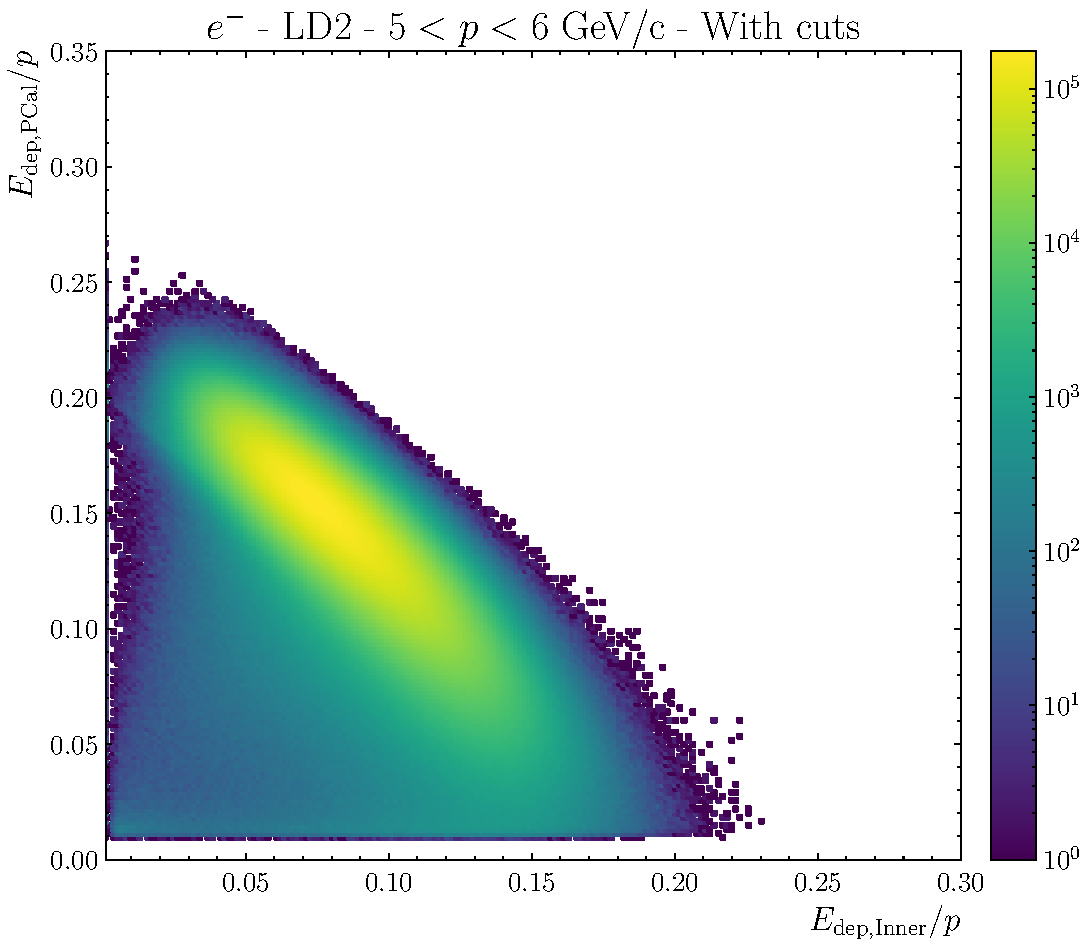
\includegraphics[width=\textwidth]{images/electron/LD2_electron_SFIn_vs_SFPcal_5_6_cuts.pdf}
    \label{fig:triangular-after}
  \end{subfigure}
  \caption{Sampling fraction of the preshower calorimeter vs sampling fraction of the inner calorimeter for electron candidate tracks in the LD2 target in outbending polarity. (a) Before any refinement cuts. (b) After all refinement cuts.}
  \label{fig:triangular-comparison}
\end{figure}

Vertex cuts are applied to ensure that selected electron tracks originate from the target region, thereby reducing background from interactions outside the target. The vertex position along the beamline ($V_z$) is used to define these cuts. 

The $V_z$ distribution for electron candidate tracks in outbending polarity is shown in \cref{fig:Vz-electron-CxC} for the three targets: LD2, CxC, and CuSn. The cuts were developed by fitting the $V_z$ distributions for the CxC and CuSn targets with two double-sided Crystal Ball (DSCB) functions for the main target peaks and two additional DSCB functions for the peaks corresponding to the empty LD2 cell walls.

\begin{figure}[hbt]
  \centering
  \begin{subfigure}[b]{0.48\textwidth}
    \centering
    \includegraphics[width=\textwidth]{images/electron/vz_e_CxC_OB_fit.pdf}
    \caption{a}
  \end{subfigure}
  \hfill
  \begin{subfigure}[b]{0.48\textwidth}
    \centering
    \includegraphics[width=\textwidth]{images/electron/vz_e_CxC_OB_fit.pdf}
    \caption{b}
  \end{subfigure}
  \caption{$V_z$ distribution for electrons in outbending polarity for the CxC (a) and CuSn (b) targets, showing the total fit and individual components.}
  \label{fig:ECAL-fiducial-cut}
\end{figure}

For the solid targets, the vertex cut ranges are defined as $\mu \pm 3\sigma$ of the main peak for each target, where $\mu$ is the mean and $\sigma$ is the standard deviation. The exception is the upper limit for CxC and Sn, which is set to 5~cm because the next peak corresponds to the scattering chamber windows, which are sufficiently far from the target region to avoid contamination. For the LD2 target, the lower limit is set to $-15$~cm to include the full target length, and the upper limit is set to 5~cm to avoid contamination from the scattering chamber windows. The resulting vertex cuts for each target in outbending polarity are summarized in \cref{tab:Vz-cuts}.

\begin{table}[htb]
\centering
\caption{Vertex cut ranges for electron candidates in outbending polarity.}
\label{tab:Vz-cuts}
\begin{tabular}{|l|c|c|}
\hline
\textbf{Target} & \textbf{$V_z$ Min (cm)} & \textbf{$V_z$ Max (cm)} \\
\hline
LD2   & $-15.0$ & $5.0$ \\
\hline
CxC   & $-10.6$ & $5.0$ \\
\hline
Cu    & $-10.6$ & $-6.5$ \\
\hline
Sn    & $-5.5$  & $5.0$ \\
\hline
\end{tabular}
\end{table}

\FloatBarrier
\subsection{Electron fiducial cuts}

To ensure uniform detector acceptance and reduce edge effects, fiducial cuts are applied to the electron candidates. These cuts define a geometric region within the detector where the response is well understood and consistent. The fiducial cuts are for the drift chambers and the calorimeter.

\subsubsection{Calorimeters fiducial cuts}
Fiducial cuts for the calorimeters are applied in the local coordinate system of each sector ($u, v$ and $w$). The RG-A Common Analysis Note provides a detailed description of the calorimeter fiducial cuts, which are implemented here without modification. The cuts are designed to exclude regions near the edges of the calorimeter sectors where the response may be non-uniform or poorly understood. For electron candidates, the fiducial cuts are $v > 9$ cm and $w > 9$ cm. It is done because the PCal bar are 4.5 cm wide, and to have a good clusters formation and reconstruction, the hit should have at least two bars. The profile of the distributions of sampling fraction as a function of $v$ and $w$ for electron candidate tracks in the LD2 target in outbending polarity are shown in \cref{fig:ECAL-fiducial-cut}. Similar plots for the CxC and CuSn targets are available in the appendix. The SF start to drop and fluctuate below 9 cm for both $v$ and $w$ coordinates.

\begin{figure}[hbt]
  \centering
  \begin{subfigure}[b]{0.48\textwidth}
    \centering
    \includegraphics[width=\textwidth]{images/electron/plots_calorimeter_fiducials/lv_vs_sf_LD2_all_sectors.pdf}
    \caption{SF vs $v$}
    \label{fig:ECAL-fiducial-cut-lv}
  \end{subfigure}
  \hfill
  \begin{subfigure}[b]{0.48\textwidth}
    \centering
    \includegraphics[width=\textwidth]{images/electron/plots_calorimeter_fiducials/lv_vs_sf_LD2_all_sectors.pdf}
    \caption{SF vs $w$}
    \label{fig:ECAL-fiducial-cut-lw}
  \end{subfigure}
  \caption{Profile of the 2D distribution SF vs $v$ (a) and $w$ (b) for electron candidate tracks in the LD2 target in outbending polarity for each sector and the overall distribution.}
  \label{fig:ECAL-fiducial-cut}
\end{figure}

The comparison of the profile of the 2D distribution SF vs $v$ or $w$ for electron candidate tracks in outbending polarity for the three targets: LD2, CxC and CuSn is shown in \cref{fig:ECAL-fiducial-cut-comp-target}. The three targets present similar distributions and justify the use of the same fiducial cuts. 

\begin{figure}[hbt]
  \centering
  \includegraphics[width=0.5\textwidth]{images/electron/plots_calorimeter_fiducials/target_comparison/lv_vs_sf_S1_target_comparison.pdf}
  \caption{Comparison of the profile of the 2D distribution SF vs $v$ or $w$ for electron candidate tracks in outbending polarity for the three targets: LD2, CxC and CuSn.}
  \label{fig:ECAL-fiducial-cut-comp-target}
\end{figure}

\FloatBarrier
\subsubsection{DC fiducial cuts}
Fiducial cuts for the drift chambers are applied using the local variable \texttt{edge} defined in the \texttt{REC::Traj} bank. This variable represents the distance between the virtual edge of the DC (defined in the simulation) and the hit position. To define the cut value, the profile of the 2D distribution of the track $\chi^2/\text{ndf}$ versus \texttt{edge} for electron candidate tracks with outbending polarity is used for the three targets.

The methodology for determining the fiducial cut position is illustrated in \cref{fig:DC-variance-method} and employs a moving variance method. This approach identifies optimal fiducial cut positions by analyzing local stability in the $\chi^2/\text{ndf}$ distribution as a function of edge distance. The method applies a sliding window (typically 5 points) across the $\chi^2/\text{ndf}$ profile and calculates the variance within each window. In regions far from the detector edges, where tracking performance is optimal and stable, the $\chi^2/\text{ndf}$ values exhibit low variance. However, as tracks approach the physical boundaries of the drift chambers, detector inefficiencies and edge effects cause the $\chi^2/\text{ndf}$ to rise unpredictably, resulting in significantly increased local variance. By scanning from the outer edge inward and identifying the first position where variance exceeds a predefined threshold (typically 0.05), the method systematically determines the boundary between the stable detector region and the degraded edge region. This approach is particularly robust because it captures the transition point where tracking quality begins to deteriorate, rather than relying on arbitrary $\chi^2/\text{ndf}$ thresholds that may vary across different detector regions or experimental conditions.

\begin{figure}[hbt]
  \centering
  \includegraphics[width=0.7\textwidth]{images/electron/plots_chi2ndf_edge/LD2_OB/variance_method_explanation.pdf}
  \caption{Illustration of the moving variance method used to determine DC fiducial cut positions. A sliding window (typically 5 points) calculates local variance across the $\chi^2/\text{ndf}$ profile. The method scans from the outer edge inward, identifying the first position where the local variance exceeds the threshold of 0.05, marking the transition from the stable detector region to the degraded edge region.}
  \label{fig:DC-variance-method}
\end{figure}

The resulting fiducial cut for sector 1 and region 1 for the LD2 target is shown in \cref{fig:DC-fiducial-cut-comp-target}. The same procedure is applied for each sector and each target. The resulting profiles for each sector for regions 1, 2, and 3 are shown in \cref{fig:DC-fiducial-cut-comp-sector-region1}, \cref{fig:DC-fiducial-cut-comp-sector-region2}, and \cref{fig:DC-fiducial-cut-comp-sector-region3}, respectively, for the LD2 target.

\begin{figure}[hbt]
  \centering
  \makebox[\textwidth][c]{%
    \hspace{2cm}
    \begin{minipage}{\dimexpr\textwidth+\marginparwidth+\marginparsep\relax}
      \centering
      % Top row: Sector 1 Region 1 detail and Region 1 all sectors
      \begin{subfigure}[b]{0.48\linewidth}
        \centering
        \includegraphics[width=\textwidth]{images/electron/plots_chi2ndf_edge/LD2_OB/fiducial_cut_Tracks_ElectronTracks_edge_vs_chi2ndf_r1_S1_1.pdf}
        \caption{Sector 1, Region 1 detail}
        \label{fig:DC-fiducial-cut-comp-target}
      \end{subfigure}
      \hfill
      \begin{subfigure}[b]{0.48\linewidth}
        \centering
        \includegraphics[width=\textwidth]{images/electron/plots_chi2ndf_edge/LD2_OB/sector_comparison/sector_comparison_r1.pdf}
        \caption{Region 1 - all sectors}
        \label{fig:DC-fiducial-cut-comp-sector-region1}
      \end{subfigure}

      \vspace{0.5cm}

      % Bottom row: Region 2 and Region 3 all sectors
      \begin{subfigure}[b]{0.48\linewidth}
        \centering
        \includegraphics[width=\textwidth]{images/electron/plots_chi2ndf_edge/LD2_OB/sector_comparison/sector_comparison_r2.pdf}
        \caption{Region 2 - all sectors}
        \label{fig:DC-fiducial-cut-comp-sector-region2}
      \end{subfigure}
      \hfill
      \begin{subfigure}[b]{0.48\linewidth}
        \centering
        \includegraphics[width=\textwidth]{images/electron/plots_chi2ndf_edge/LD2_OB/sector_comparison/sector_comparison_r3.pdf}
        \caption{Region 3 - all sectors}
        \label{fig:DC-fiducial-cut-comp-sector-region3}
      \end{subfigure}
    \end{minipage}%
  }
  \caption{DC fiducial cuts for electron candidate tracks in outbending polarity for the LD2 target. (a) Application of the moving variance method for sector 1, region 1, showing the $\chi^2/\text{ndf}$ profile with the local variance calculation and the resulting fiducial cut position where variance exceeds the 0.05 threshold. (b-d) Profiles of $\chi^2/\text{ndf}$ vs \texttt{edge} for all sectors in regions 1, 2, and 3, respectively, with determined fiducial cut positions indicated.}
  \label{fig:DC-fiducial-cuts-combined}
\end{figure}

To validate the robustness of the DC fiducial cuts, the dependence of the $\chi^2/\text{ndf}$ profiles on electron momentum and scattering angle is investigated. The $\chi^2/\text{ndf}$ versus \texttt{edge} profiles are examined in different momentum bins (0.5-2 GeV, 2-4 GeV, 4-6 GeV, and $>$6 GeV) for each region, as shown in \cref{fig:DC-momentum-dep-r1,fig:DC-momentum-dep-r2,fig:DC-momentum-dep-r3}. The profiles remain consistent across momentum ranges, with the fiducial cut positions showing minimal momentum dependence. This indicates that the single fiducial cut value determined from the integrated momentum distribution is appropriate for all electron momenta.

\begin{figure}[hbt]
  \begin{minipage}{\dimexpr\textwidth+\marginparwidth+\marginparsep\relax}
    \centering
    \begin{subfigure}[b]{0.32\linewidth}
      \centering
      \includegraphics[width=\textwidth]{images/electron/plots_chi2ndf_edge/LD2_OB/momentum_bins/momentum_comparison_r1.pdf}
      \caption{Region 1}
      \label{fig:DC-momentum-dep-r1}
    \end{subfigure}
    \hfill
    \begin{subfigure}[b]{0.32\linewidth}
      \centering
      \includegraphics[width=\textwidth]{images/electron/plots_chi2ndf_edge/LD2_OB/momentum_bins/momentum_comparison_r2.pdf}
      \caption{Region 2}
      \label{fig:DC-momentum-dep-r2}
    \end{subfigure}
    \hfill
    \begin{subfigure}[b]{0.32\linewidth}
      \centering
      \includegraphics[width=\textwidth]{images/electron/plots_chi2ndf_edge/LD2_OB/momentum_bins/momentum_comparison_r3.pdf}
      \caption{Region 3}
      \label{fig:DC-momentum-dep-r3}
    \end{subfigure}
  \end{minipage}
  \caption{Momentum dependence of DC fiducial cuts for the LD2 target in outbending polarity. The $\chi^2/\text{ndf}$ vs \texttt{edge} profiles are shown for different momentum bins in regions 1, 2, and 3, demonstrating consistent behavior across the full momentum range.}
  \label{fig:DC-momentum-dependence}
\end{figure}

Similarly, the angular dependence is studied by binning the data in polar angle $\theta$ ranges corresponding to different detector geometries. As shown in \cref{fig:DC-theta-dep-r1,fig:DC-theta-dep-r2,fig:DC-theta-dep-r3}, the $\chi^2/\text{ndf}$ profiles exhibit consistent behavior across different $\theta$ bins within each region. The slight variations observed are within the statistical uncertainties and do not require $\theta$-dependent fiducial cuts.

\begin{figure}[hbt]
  \begin{minipage}{\dimexpr\textwidth+\marginparwidth+\marginparsep\relax}
    \centering
    \begin{subfigure}[b]{0.32\linewidth}
      \centering
      \includegraphics[width=\textwidth]{images/electron/plots_chi2ndf_edge/LD2_OB/theta_bins/theta_comparison_r1.pdf}
      \caption{Region 1}
      \label{fig:DC-theta-dep-r1}
    \end{subfigure}
    \hfill
    \begin{subfigure}[b]{0.32\linewidth}
      \centering
      \includegraphics[width=\textwidth]{images/electron/plots_chi2ndf_edge/LD2_OB/theta_bins/theta_comparison_r2.pdf}
      \caption{Region 2}
      \label{fig:DC-theta-dep-r2}
    \end{subfigure}
    \hfill
    \begin{subfigure}[b]{0.32\linewidth}
      \centering
      \includegraphics[width=\textwidth]{images/electron/plots_chi2ndf_edge/LD2_OB/theta_bins/theta_comparison_r3.pdf}
      \caption{Region 3}
      \label{fig:DC-theta-dep-r3}
    \end{subfigure}
  \end{minipage}
  \caption{Angular dependence of DC fiducial cuts for the LD2 target in outbending polarity. The $\chi^2/\text{ndf}$ vs \texttt{edge} profiles are shown for different $\theta$ bins in regions 1, 2, and 3, showing consistent edge effects independent of scattering angle.}
  \label{fig:DC-theta-dependence}
\end{figure}

The DC fiducial cuts are also compared across the three different targets (LD2, CxC, and CuSn) for sector 1 in each region, as shown in \cref{fig:DC-target-comp-r1,fig:DC-target-comp-r2,fig:DC-target-comp-r3}. The profiles are nearly identical for all three targets, with fiducial cut positions differing by less than 0.1 cm on average (see \cref{tab:fiducial_cuts}). This similarity justifies using the same DC fiducial cut methodology across all targets.

\begin{figure}[hbt]
  \begin{minipage}{\dimexpr\textwidth+\marginparwidth+\marginparsep\relax}
    \centering
    \begin{subfigure}[b]{0.32\linewidth}
      \centering
      \includegraphics[width=\textwidth]{images/electron/plots_chi2ndf_edge/target_comparison/OB/target_comparison_r1_S1.pdf}
      \caption{Region 1}
      \label{fig:DC-target-comp-r1}
    \end{subfigure}
    \hfill
    \begin{subfigure}[b]{0.32\linewidth}
      \centering
      \includegraphics[width=\textwidth]{images/electron/plots_chi2ndf_edge/target_comparison/OB/target_comparison_r2_S1.pdf}
      \caption{Region 2}
      \label{fig:DC-target-comp-r2}
    \end{subfigure}
    \hfill
    \begin{subfigure}[b]{0.32\linewidth}
      \centering
      \includegraphics[width=\textwidth]{images/electron/plots_chi2ndf_edge/target_comparison/OB/target_comparison_r3_S1.pdf}
      \caption{Region 3}
      \label{fig:DC-target-comp-r3}
    \end{subfigure}
  \end{minipage}
  \caption{Target comparison of DC fiducial cuts for sector 1 in outbending polarity. The $\chi^2/\text{ndf}$ vs \texttt{edge} profiles for LD2, CxC, and CuSn targets are nearly identical across all three regions, demonstrating target-independent edge effects.}
  \label{fig:DC-target-comparison}
\end{figure}

The average fiducial cut positions for each region for the outbending polarity are summarized in \cref{tab:fiducial_cuts}.

\begin{table}[htbp]
\centering
\caption{Average Fiducial Cut Positions by Region for the outbending polarity.}
\label{tab:fiducial_cuts}
\begin{tabular}{|c|c|c|}
\hline
\textbf{Region 1} (cm) & \textbf{Region 2} (cm) & \textbf{Region 3} (cm) \\
\hline
 $1.88\pm0.16$ & $2.08 \pm 0.10$ & $8.62 \pm 0.55$  \\
\hline
\end{tabular}
\end{table}

\FloatBarrier
\section{Summary}

Here is a table that recapitulates all the cuts: 
\begin{table}[htb]
\centering
\begin{tabular}{|l|l|l|}
\hline
\textbf{Cut Type} & \textbf{Cut Description} & \textbf{Value/Requirement} \\
\hline
Particle ID & Event Builder assignment & $\texttt{pid} = 11$ (electron) \\
\hline
Status & Forward Detector trigger & $-4000 < \texttt{status} \leq -2000$ \\
\hline
Momentum & Minimum momentum & $p > 0.8$ GeV \\
\hline
SF vs Momentum & Momentum-dependent SF & $\mu_{\text{SF}} \pm 3.5\sigma$ vs $p$ \\
\hline
Calorimeter $v,w$ coordinate & Local coordinate cut & $v,w > 9$ cm \\
\hline
Drift Chamber Edge & Distance from DC edge & \texttt{edge} $> $ region dependent \\
\hline
Vertex $V_z$ & Target vertex position & Target dependent (see \cref{tab:Vz-cuts}) \\
\hline
\end{tabular}
\caption{Summary of all cuts applied for electron identification and selection in RG-D analysis.}
\label{tab:electron-cuts-summary}
\end{table}

The survival rates after each cut for the different targets are summarized in \cref{tab:cut_efficiencies}.
\begin{table}[htb]
\centering
\label{tab:cut_efficiencies}
\begin{tabular}{|l|l|c|c|c|}
\hline
\textbf{Target} & \textbf{Cut} & \textbf{Cumulative} & \textbf{Step} \\
\hline
\multirow{5}{*}{LD2} 
    & Momentum cut              & 1.0000 & 1.0000 \\
    & Sampling fraction cut     & 0.9714 & 0.9715 \\
    & PCAL cut                  & 0.9714 & 1.0000 \\
    & DC cut                    & 0.9522 & 0.9802 \\
    & Vz cut                    & 0.8995 & 0.9447 \\
\hline
\multirow{5}{*}{CxC} 
    & Momentum cut              & 1.0000 & 1.0000 \\
    & Sampling fraction cut     & 0.9740 & 0.9740 \\
    & PCAL cut                  & 0.9740 & 1.0000 \\
    & DC cut                    & 0.9550 & 0.9805 \\
    & Vz cut                    & 0.7779 & 0.8146 \\
\hline
\multirow{4}{*}{CuSn} 
    & Momentum cut              & 1.0000 & 1.0000 \\
    & Sampling fraction cut     & 0.9824 & 0.9824 \\
    & PCAL cut                  & 0.9823 & 0.9999 \\
    & DC cut                    & 0.9642 & 0.9816 \\
\hline
\end{tabular}
\caption{Electron survival rates for different targets}
\end{table}


\section{Pion cuts}
Pion identification and selection are necessery for the color transparancy study and the nuclear TMDs analysis in RG-D. The pion selection is done by applying cuts on the reconstructed mass of the particle, calculated using the time-of-flight information from the time-of-flight detectors and the momentum from the drift chambers.

The fiducial cuts for the drift chambers and the calorimeter will be descripted in the next subsections.

\subsection{DC fiducial cuts}
The same methodology as for the electron DC fiducial cuts is applied for the pion candidate tracks. The resulting profiles for each sector for regions 1, 2, and 3 are shown for the sector average in \cref{fig:DC-fiducial-cut-pion-LD2}, \cref{fig:DC-fiducial-cut-pion-CxC}, and \cref{fig:DC-fiducial-cut-pion-CuSn}, respectively, for the LD2 target.

For $\pi^-$, the optimal cut positions are 2.125~cm, 3.625~cm, and 9.625~cm for regions 1, 2, and 3, respectively. For $\pi^+$, the cut positions are 3.875~cm, 4.375~cm, and 2.625~cm for regions 1, 2, and 3, respectively.


\begin{figure}[hbt]
  \centering
  \begin{subfigure}[b]{\textwidth}
    \centering
    \includegraphics[width=\textwidth]{images/pions/LD2_OB/pion_charge_comparison.pdf}
    \caption{LD2}
    \label{fig:DC-fiducial-cut-pion-LD2}
  \end{subfigure}
  \vfill
  \begin{subfigure}[b]{\textwidth}
    \centering
    \includegraphics[width=\textwidth]{images/pions/CxC_OB/pion_charge_comparison.pdf}
    \caption{CxC}
    \label{fig:DC-fiducial-cut-pion-CxC}
  \end{subfigure}
  \vfill
  \begin{subfigure}[b]{\textwidth}
    \centering
    \includegraphics[width=\textwidth]{images/pions/CuSn_OB/pion_charge_comparison.pdf}
    \caption{CuSn}
    \label{fig:DC-fiducial-cut-pion-CuSn}
  \end{subfigure}
  \caption{DC fiducial cuts for pion candidate tracks in outbending polarity for the three targets (sector average).}
\end{figure}

\FloatBarrier

\subsection{PCal fiducial cuts}
The PCal fiducial cuts for pions are applied to remove tracks that are close to the edges of the calorimeter, where the reconstruction efficiency is lower. The cuts are based on the local coordinates $l_v$ and $l_w$ of the track in the PCal. The distributions of the sampling fraction as a function of $l_v$ and $l_w$ are shown in \cref{fig:PCal-fiducial-cut-pion-lv} and \cref{fig:PCal-fiducial-cut-pion-lw}, respectively. The fiducial cuts are $l_v > 14$~cm and $l_w > 14$~cm.

\begin{figure}[hbt]
  \centering
  \includegraphics[width=0.7\textwidth]{images/pions/lv_vs_sf_LD2_particles.pdf}
  \caption{Sampling fraction as a function of $l_v$ for pion candidates in the LD2 target.}
  \label{fig:PCal-fiducial-cut-pion-lv}
\end{figure}

\begin{figure}[hbt]
  \centering
  \includegraphics[width=0.7\textwidth]{images/pions/lw_vs_sf_LD2_particles.pdf}
  \caption{Sampling fraction as a function of $l_w$ for pion candidates in the LD2 target.}
  \label{fig:PCal-fiducial-cut-pion-lw}
\end{figure}

\FloatBarrier
\newpage
\clearpage

\appendix

\section{Sector Parameters}

\subsection*{Outbending (OB)}
\begin{table}[h]
\tiny
\centering
\caption{Sampling fraction polynomial parameters for outbending polarity.} \label{tab:sf-params-ob}
\begin{tabular}{|c|c|c|c|c|c|c|c|c|c|}
\hline
\textbf{Target} & \textbf{Sector} & \textbf{$a_\mu$} & \textbf{$b_\mu$} & \textbf{$c_\mu$} & \textbf{$d_\mu$} & \textbf{$a_\sigma$} & \textbf{$b_\sigma$} & \textbf{$c_\sigma$} & \textbf{$d_\sigma$} \\ \hline
\multirow{6}{*}{LD2} & S1 & 2.284817E-01 & 5.741607E-03 & -7.956694E-04 & 2.165831E-05 & 2.278400E-02 & -3.478097E-03 & 3.644345E-04 & -1.564506E-05 \\ \cline{2-10}
& S2 & 2.272353E-01 & 6.035907E-03 & -5.379217E-04 & -1.432191E-06 & 2.214450E-02 & -2.992410E-03 & 2.810789E-04 & -1.021893E-05 \\ \cline{2-10}
& S3 & 2.248222E-01 & 9.544562E-03 & -1.331928E-03 & 4.146476E-05 & 2.455364E-02 & -4.547263E-03 & 5.091026E-04 & -2.082045E-05 \\ \cline{2-10}
& S4 & 2.262726E-01 & 6.742876E-03 & -6.707265E-04 & 6.027435E-06 & 2.270259E-02 & -3.090211E-03 & 2.849498E-04 & -1.108599E-05 \\ \cline{2-10}
& S5 & 2.294593E-01 & 3.253914E-03 & -6.716294E-05 & -2.106351E-05 & 2.353437E-02 & -4.471507E-03 & 5.546300E-04 & -2.564773E-05 \\ \cline{2-10}
& S6 & 2.248109E-01 & 7.709680E-03 & -9.387105E-04 & 1.955346E-05 & 2.320134E-02 & -3.707398E-03 & 4.086606E-04 & -1.827203E-05 \\ \hline
\multirow{6}{*}{CxC} & S1 & 2.297164E-01 & 4.850482E-03 & -6.473612E-04 & 1.386706E-05 & 2.160027E-02 & -2.804498E-03 & 2.481187E-04 & -9.444168E-06 \\ \cline{2-10}
& S2 & 2.284924E-01 & 5.444945E-03 & -4.057949E-04 & -9.745369E-06 & 2.097248E-02 & -2.301250E-03 & 1.681611E-04 & -4.820942E-06 \\ \cline{2-10}
& S3 & 2.257831E-01 & 8.799251E-03 & -1.210729E-03 & 3.520214E-05 & 2.364466E-02 & -3.974250E-03 & 4.048261E-04 & -1.517698E-05 \\ \cline{2-10}
& S4 & 2.290273E-01 & 4.774422E-03 & -3.194710E-04 & -1.291518E-05 & 2.131817E-02 & -2.278156E-03 & 1.421861E-04 & -3.384835E-06 \\ \cline{2-10}
& S5 & 2.312938E-01 & 1.779729E-03 & 1.881011E-04 & -3.479554E-05 & 2.238608E-02 & -3.777670E-03 & 4.241412E-04 & -1.815833E-05 \\ \cline{2-10}
& S6 & 2.271200E-01 & 6.051471E-03 & -6.286571E-04 & 1.997614E-06 & 2.170337E-02 & -2.868470E-03 & 2.639296E-04 & -1.041341E-05 \\ \hline
\multirow{6}{*}{CuSn} & S1 & 2.320707E-01 & 3.994131E-03 & -4.894629E-04 & 1.898325E-06 & 2.241820E-02 & -3.277630E-03 & 3.136628E-04 & -1.234151E-05 \\ \cline{2-10}
& S2 & 2.302078E-01 & 3.476050E-03 & -1.567172E-04 & -2.212723E-05 & 2.141103E-02 & -2.354403E-03 & 1.075100E-04 & 1.855098E-06 \\ \cline{2-10}
& S3 & 2.268107E-01 & 8.877708E-03 & -1.179578E-03 & 3.071273E-05 & 2.378785E-02 & -4.104492E-03 & 4.372052E-04 & -1.750814E-05 \\ \cline{2-10}
& S4 & 2.290050E-01 & 6.702587E-03 & -7.847463E-04 & 1.459749E-05 & 2.250505E-02 & -2.997400E-03 & 2.528880E-04 & -8.680370E-06 \\ \cline{2-10}
& S5 & 2.298645E-01 & 4.027068E-03 & -2.501656E-04 & -1.062495E-05 & 2.240025E-02 & -3.576763E-03 & 3.577542E-04 & -1.355748E-05 \\ \cline{2-10}
& S6 & 2.268440E-01 & 6.788151E-03 & -8.409054E-04 & 1.710382E-05 & 2.268680E-02 & -3.427790E-03 & 3.396480E-04 & -1.371903E-05 \\ \hline
\multirow{6}{*}{Average} & S1 & 2.300896E-01 & 4.862074E-03 & -6.441645E-04 & 1.247456E-05 & 2.226749E-02 & -3.186742E-03 & 3.087387E-04 & -1.247691E-05 \\ \cline{2-10}
& S2 & 2.286452E-01 & 4.985634E-03 & -3.668113E-04 & -1.110160E-05 & 2.150934E-02 & -2.549354E-03 & 1.855833E-04 & -4.394923E-06 \\ \cline{2-10}
& S3 & 2.258053E-01 & 9.073840E-03 & -1.240745E-03 & 3.579321E-05 & 2.399538E-02 & -4.208668E-03 & 4.503779E-04 & -1.783519E-05 \\ \cline{2-10}
& S4 & 2.281016E-01 & 6.073295E-03 & -5.916479E-04 & 2.569914E-06 & 2.217527E-02 & -2.788589E-03 & 2.266746E-04 & -7.717066E-06 \\ \cline{2-10}
& S5 & 2.302059E-01 & 3.020237E-03 & -4.307581E-05 & -2.216133E-05 & 2.277357E-02 & -3.941980E-03 & 4.455085E-04 & -1.912118E-05 \\ \cline{2-10}
& S6 & 2.262583E-01 & 6.849767E-03 & -8.027577E-04 & 1.288497E-05 & 2.253050E-02 & -3.334553E-03 & 3.374127E-04 & -1.413483E-05 \\ \hline
\end{tabular}
\end{table}

\subsection*{Inbending (IB)}
\begin{table}[h]
\tiny
\centering
\caption{Sampling fraction polynomial parameters for inbending polarity.} \label{tab:sf-params-ib}
\begin{tabular}{|c|c|c|c|c|c|c|c|c|c|}
\hline
\textbf{Target} & \textbf{Sector} & \textbf{$a_\mu$} & \textbf{$b_\mu$} & \textbf{$c_\mu$} & \textbf{$d_\mu$} & \textbf{$a_\sigma$} & \textbf{$b_\sigma$} & \textbf{$c_\sigma$} & \textbf{$d_\sigma$} \\ \hline
\multirow{6}{*}{LD2} & S1 & 2.311090E-01 & 4.309850E-03 & -5.451468E-04 & 4.964926E-06 & 2.235234E-02 & -3.117219E-03 & 2.887163E-04 & -1.130302E-05 \\ \cline{2-10}
& S2 & 2.304337E-01 & 3.585701E-03 & -1.672183E-04 & -2.195166E-05 & 2.170119E-02 & -2.428043E-03 & 1.302137E-04 & -2.341453E-09 \\ \cline{2-10}
& S3 & 2.269121E-01 & 8.797654E-03 & -1.171428E-03 & 3.051411E-05 & 2.423452E-02 & -4.301838E-03 & 4.742717E-04 & -1.982933E-05 \\ \cline{2-10}
& S4 & 2.288870E-01 & 6.786554E-03 & -8.022669E-04 & 1.557290E-05 & 2.313618E-02 & -3.260224E-03 & 3.018553E-04 & -1.156727E-05 \\ \cline{2-10}
& S5 & 2.288645E-01 & 4.637371E-03 & -3.662910E-04 & -4.233388E-06 & 2.310886E-02 & -3.892809E-03 & 4.115044E-04 & -1.656696E-05 \\ \cline{2-10}
& S6 & 2.272092E-01 & 6.581994E-03 & -8.197215E-04 & 1.632205E-05 & 2.321750E-02 & -3.665701E-03 & 3.804620E-04 & -1.587632E-05 \\ \hline
\multirow{6}{*}{CxC} & S1 & 2.311089E-01 & 4.309932E-03 & -5.451631E-04 & 4.965863E-06 & 2.235235E-02 & -3.117219E-03 & 2.887137E-04 & -1.130271E-05 \\ \cline{2-10}
& S2 & 2.304337E-01 & 3.585739E-03 & -1.672262E-04 & -2.195117E-05 & 2.170108E-02 & -2.427968E-03 & 1.302009E-04 & -1.715883E-09 \\ \cline{2-10}
& S3 & 2.269124E-01 & 8.797523E-03 & -1.171404E-03 & 3.051277E-05 & 2.423476E-02 & -4.301977E-03 & 4.742961E-04 & -1.983062E-05 \\ \cline{2-10}
& S4 & 2.288871E-01 & 6.786452E-03 & -8.022473E-04 & 1.557178E-05 & 2.313635E-02 & -3.260315E-03 & 3.018706E-04 & -1.156805E-05 \\ \cline{2-10}
& S5 & 2.288645E-01 & 4.637396E-03 & -3.662963E-04 & -4.233103E-06 & 2.310898E-02 & -3.892887E-03 & 4.115187E-04 & -1.656775E-05 \\ \cline{2-10}
& S6 & 2.272093E-01 & 6.581935E-03 & -8.197067E-04 & 1.632106E-05 & 2.321749E-02 & -3.665704E-03 & 3.804646E-04 & -1.587659E-05 \\ \hline
\multirow{6}{*}{CuSn} & S1 & 2.311087E-01 & 4.310017E-03 & -5.451781E-04 & 4.966680E-06 & 2.235247E-02 & -3.117310E-03 & 2.887315E-04 & -1.130379E-05 \\ \cline{2-10}
& S2 & 2.304337E-01 & 3.585708E-03 & -1.672224E-04 & 2.195131E-05 & 2.170126E-02 & -2.428101E-03 & 1.302294E-04 & -3.452408E-09 \\ \cline{2-10}
& S3 & 2.269123E-01 & 8.797570E-03 & -1.171414E-03 & 3.051337E-05 & 2.423472E-02 & -4.301969E-03 & 4.742963E-04 & -1.983071E-05 \\ \cline{2-10}
& S4 & 2.288870E-01 & 6.786555E-03 & -8.022665E-04 & 1.557285E-05 & 2.313625E-02 & -3.260272E-03 & 3.018643E-04 & -1.156777E-05 \\ \cline{2-10}
& S5 & 2.288646E-01 & 4.637320E-03 & -3.662803E-04 & -4.234038E-06 & 2.310900E-02 & -3.892931E-03 & 4.115288E-04 & -1.656837E-05 \\ \cline{2-10}
& S6 & 2.272092E-01 & 6.582013E-03 & -8.197249E-04 & 1.632221E-05 & 2.321744E-02 & -3.665649E-03 & 3.804500E-04 & -1.587559E-05 \\ \hline
\multirow{6}{*}{Average} & S1 & 2.311088E-01 & 4.309933E-03 & -5.451627E-04 & 4.965823E-06 & 2.235239E-02 & -3.117249E-03 & 2.887205E-04 & -1.130317E-05 \\ \cline{2-10}
& S2 & 2.304337E-01 & 3.585716E-03 & -1.672223E-04 & -7.317175E-06 & 2.170118E-02 & -2.428037E-03 & 1.302147E-04 & -2.503248E-09 \\ \cline{2-10}
& S3 & 2.269123E-01 & 8.797582E-03 & -1.171416E-03 & 3.051342E-05 & 2.423467E-02 & -4.301928E-03 & 4.742880E-04 & -1.983022E-05 \\ \cline{2-10}
& S4 & 2.288870E-01 & 6.786520E-03 & -8.022602E-04 & 1.557251E-05 & 2.313626E-02 & -3.260271E-03 & 3.018634E-04 & -1.156770E-05 \\ \cline{2-10}
& S5 & 2.288645E-01 & 4.637362E-03 & -3.662892E-04 & -4.233509E-06 & 2.310895E-02 & -3.892876E-03 & 4.115173E-04 & -1.656769E-05 \\ \cline{2-10}
& S6 & 2.272093E-01 & 6.581981E-03 & -8.197177E-04 & 1.632178E-05 & 2.321748E-02 & -3.665685E-03 & 3.804588E-04 & -1.587616E-05 \\ \hline
\end{tabular}
\end{table}



\section{Number of photo-electrons in HTCC}

\begin{figure}[hbt]
  \centering
  \includegraphics[width=1.3\textwidth]{images/electron/plots_event_builder/nphe_neg_all_targets_IB.pdf}
  \caption{HTCC photo-electron distribution for all negative tracks in the Forward Detector in inbending polarity for the torus, apply cut at $N_{\text{phe}} > 2$ for pion rejection.}
  \label{fig:nphe-IB}
\end{figure}

\section{Sampling fraction versus momentum}
\begin{figure}[hbt]
  \centering
  \includegraphics[width=0.7\textwidth]{images/electron/plots_sampling_fraction/OB/sectors_comparison_CxC.pdf}
  \caption{Comparison of the sampling fraction mean and sigma as a function of momentum for the CxC target in outbending polarity for different sectors and the overall distribution.}
  \label{fig:SF-CxC-comparison}
\end{figure}

\begin{figure}[hbt]
  \centering
  \includegraphics[width=0.7\textwidth]{images/electron/plots_sampling_fraction/OB/sectors_comparison_CuSn.pdf}
  \caption{Comparison of the sampling fraction mean and sigma as a function of momentum for the CuSn target in outbending polarity for different sectors and the overall distribution.}
  \label{fig:SF-CuSn-comparison}
\end{figure}


\section{Calorimeter fiducial cuts}
\begin{figure}[hbt]
  \centering
  \includegraphics[width=0.7\textwidth]{images/electron/plots_calorimeter_fiducials/lv_vs_sf_CxC_all_sectors.pdf}
  \caption{Profile of the 2D distribution SF vs $v$ or $w$ for electron candidate tracks in the CxC target in outbending polarity for each sectors and the overall distribution.}
  \label{fig:ECAL-CxC-fiducial-cut}
\end{figure}


\begin{figure}[hbt]
  \centering
  \includegraphics[width=0.7\textwidth]{images/electron/plots_calorimeter_fiducials/lv_vs_sf_CuSn_all_sectors.pdf}
  \caption{Profile of the 2D distribution SF vs $v$ or $w$ for electron candidate tracks in the CuSn target in outbending polarity for each sectors and the overall distribution.}
  \label{fig:ECAL-CuSn-fiducial-cut}
\end{figure}



\end{document}